	Bei der Auger-Elektronen-Spektroskopie (auch AES) handelt es sich um ein Oberflächenanalyseverfahren.
	Dieses kann sowohl qualitative als auch quantitative Aussagen über die Zusammensetzung der Probe machen. 
	Wie der Name schon sagt, wird vor Allem der sogenannte Auger-Effekt ausgenutzt, um durch Messung auf das Vorkommen von Elementen zu schließen.

\subsection{Auger-Effekt} % (fold)
\label{sub:auger_effekt}

	Der Auger-Effekt beruht auf dem strahlungsfreien Übergang der Elektronen in der Elektronenhülle eines Atoms.
	Er kann anschaulich durch folgenden Prozess, welcher auch Auger-Prozess genannt wird, erklärt werden:
	
	\begin{itemize}
		\item
			Durch externe Anregung wird ein stark-gebundenes Elektron auf einer der inneren Schalen des Atoms ionisiert.
			Dies kann durch Röntgenstrahlung oder anderen Elektronen geschehen.
		\item
			Der freie Platz wird nun, aufgrund der niederenergetischen Lage, durch ein Elektron einer höheren Schale besetzt (auch Relaxation).
		\item
			Frei-werdende Energie, welche durch diesen Übergang entsteht, kann entweder in Form von Röntgenstrahlung oder aber strahlungsfrei an ein Elektron einer höheren Schale abgegeben werden.
			Dieses Elektron wird auch Auger-Elektron genannt.
		\item
			Findet ein strahlungsfreier Übergang statt und besitzt das Auger-Elektron genügend Energie, um die Austrittsarbeit des Festkörpers zu überwinden, so verlässt es diesen.
			Das Atom ist damit zweifach-positiv geladen. 
			Dieser Effekt wird auch der Auger-Effekt genannt.
	\end{itemize}

	Damit wird klar, dass ein Auger-Elektron nur bei Atomen mit mehr als zwei Elektronen beobachtet werden kann. 
	Es lassen sich also Wasserstoff (H) und Helium (He) nicht nachweisen. \cite{description}\\

	Einzelne Auger-Prozesse werden auch durch die vorkommenden Elektronenschalen und deren Reihenfolge charakterisiert.
	Zum Beispiel handelt es sich bei einem KLL-Prozess um einen Auger-Prozess, bei dem das erste Elektronen aus der innersten K-Schale ionisiert wurde, 
	das zweite Elektronen aus der darüber liegenden L-Schale den Platz einnahm und das dritte Elektron ebenfalls aus der L-Schale zum Auger-Elektron wurde.

	Es sei hier gesagt, dass die Wahrscheinlichkeit eines Auger-Prozesses, bei dem Relaxation und Emission derselben Schale entspringt, größer ist (Beispiele: KLL, LMM, MNN). \cite{description}\\

	Seien nun $W,X,Y$ drei beliebige Elektronenschalen eines Atoms mit $W < X \leq Y$. 
	Sei weiterhin die Kernladungszahl $Z$ und die Austrittsarbeit $\Phi_A$. 
	Dann gilt nach voriger Betrachtung für die Energie $E_{WXY}$ eines Auger-Elektrons:
	\[
		E_{WXY} = E_W(Z) - E_X(Z+\Delta Z) - E_Y(Z+\Delta Z) - \Phi_A
	\]
	Hierbei repräsentiert $E_i(Z)$ die Energie der $i$.ten-Schale zur Kernladungszahl $Z$.
	Es muss beachtet werden, dass sich die Kernladungszahl um $\Delta Z$ während des Auger-Prozesses verändert. \cite{article} \\

	Wie bereits erwähnt, kann durch die externe Anregung auch Röntgenstrahlung entstehen.
	Die Wahrscheinlichkeit für die Entstehung dieser ist proportional zu $Z^4$, wobei $Z$ die Kernladungszahl ist.
	Folglich entstehen Auger-Elektronen eher bei leichten und Röntgenstrahlen eher bei schweren Atomen. \cite{description} \\

	Die Ermittlung der chemischen Zusammensetzung durch die AES beruht auf der Messung der charakteristischen kinetischen Energien der Auger-Elektronen. 
	Aufgrund der inelastischen Wechselwirkungen im Festkörper verlieren diese jedoch an Energie. 
	Die Streuung innerhalb der Probe bestimmt somit die Austrittstiefe und dadurch ebenfalls die Oberflächenempfindlichkeit.
	Die Austrittstiefe wird durch die inelastische mittlere freie Weglänge charakterisiert, welche die zurückgelegte Strecke zwischen zwei inelastischen Stößen angibt.
	Im Normalfall liegt sie bei ungefähr zehn Monolagen, wobei sie von mehreren Größen abhängt (Beispiel: kinetische Energie der Elektronen). \cite{description}


% subsection auger_effekt (end)

\subsection{Grundprinzip der AES} % (fold)
\label{sub:grundprinzip_der_aes}

	Durch Elektronenbeschuss werden die kernnahen Elektronen ausgelöst und der Auger-Prozess kann statt finden. 
	Anschließend werden die von der Probe zurückkommenden Elektronen mit Hilfe eines Detektors nachgewiesen. 
	Folglich können elastisch rückgestreute Primärelektronen, Sekundärelektronen und Auger-Elektronen energiedispersiv detektiert werden.
	Trägt man die Anzahl der detektierten Elektronen über deren kinetischen Energie von Null bis hin zur Anregungsenergie auf, so erhält man Auger-Spektren.
	Wichtig ist dabei, dass das erhaltene Signal lediglich proportional zur Anzahl der Elektronen ist und keinen Absolutwert darstellt. \cite{description}
	Anhand der folgenden Abbildung wird ersichtlich, dass die Auger-Peaks eher klein im Vergleich zu den anderen auftretenden Erscheinungen sind. 

	\begin{figure}[h]
		\centering
		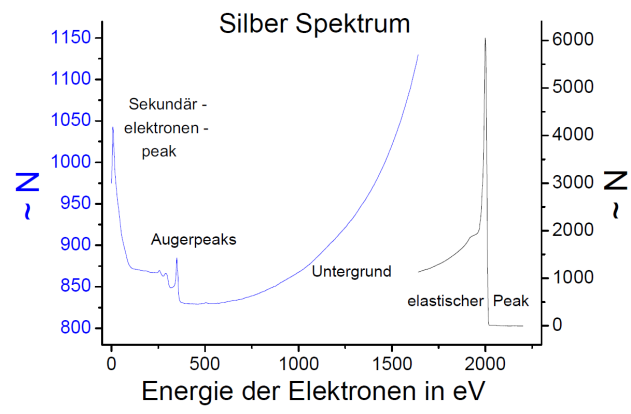
\includegraphics[scale=0.6]{Ag-Spektrum.png}
		\caption{Auger-Spektrum von Silber (Ag) \cite{description}}
	\end{figure}


% subsection grundprinzip_der_aes (end)

\subsection{chemische Verschiebung} % (fold)
\label{sub:chemische_verschiebung}

	Die kinetische Energie der Auger-Elektronen wird nicht nur von der Atomsorte selbst beeinflusst, sondern auch von der chemischen Umgebung des Atoms. 
	Eine reine Elementprobe erzeugt andere Werte, als die gleichen Atome in einer Verbindung.
	Die chemischen Bindungen führen zu einer Veränderung der Elektronenniveaus durch Ladungstransfer und damit auch zu geänderten Bindungsenergien. 
	Das Vorzeichen der chemischen Verschiebung ist für alle Energieniveaus einer Atomsorte gleich.
	Abbildung \ref{chemshift} zeigt dies am Beispiel von Silizium (Si). \cite{description}

	\begin{figure}[h]
		\centering
		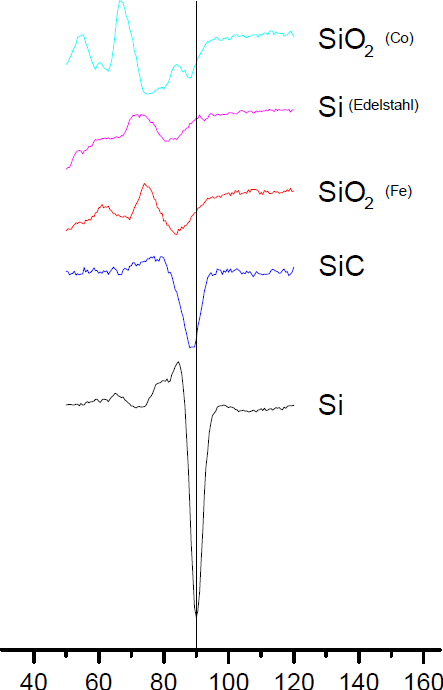
\includegraphics[scale=0.4]{chem-shift.png}
		\caption{Chemische Verschiebung des Silizium-LMM-Peaks \cite{description}}
		\label{chemshift}
	\end{figure}


% subsection chemische_verschiebung (end)

\subsection{Relativer Empfindlichkeitsfaktor} % (fold)
\label{sub:relativer_empfindlichkeitsfaktor}

	Vermisst man zwei verschiedene Elemente gleicher Konzentration mit den gleichen Parametern, so erhält man im Allgemeinen unterschiedliche Peakintensitäten. 
	Der Zusammenhang zwischen den Peakintensitäten und den physikalischen Größen ist nicht ohne größeren Aufwand mathematisch quantifizierbar.
	Um dennoch einen Vergleich der Intensitäten ermöglichen zu können, behilft man sich	mit einem empirischen Faktor.
	Dieser Faktor wird auch relativer Empfindlichkeitsfaktor $S$ genannt. 
	Hierbei wird die Intensität des untersuchten Stoffes mit der eines Vergleichselements normiert. 
	Im Allgemeinen hat sich der 351eV Auger-Peak von Silber als Referenz etabliert.
	Damit gilt für Silber (Ag):
	\[ 
		S(Ag) = 1 
	\]
	Der relative Empfindlichkeitsfaktor wurde für verschiedene Anregungsenergien bestimmt und tabelliert.
	Nicht jedes Element ist jedoch in reiner Form messbar, weshalb man sich mit verschiedenen Verbindungen behilft. 
	Untersucht man eine Probe der Verbindung $X_AY_B$, wobei $X,Y$ Elemente und $A,B$ Stöchometriefaktoren sind, so gilt:
	\[ 
		S(X) = \dfrac{A+B}{A}\cdot \dfrac{I(X)}{I(Ag)} 
	\]
	Hierbei bezeichnet $I$ die gemessene Intensität (Peak-Peak-Amplitude) des jeweiligen Stoffes. \cite{description}

% subsection relativer_empfindlichkeitsfaktor (end)

\subsection{Quantitative Analyse} % (fold)
\label{sub:quantitative_analyse}

	Seien nun $A$ die Menge der Elemente einer untersuchten Probe und $X \in A$. 
	Dann lässt sich aufgrund der vorherigen Betrachtung folgendes über die relative Konzentration $c$ von $X$ sagen:
	\[
		c(X) = \dfrac{I(X)}{S(X)}\cdot\left( \sum_{\alpha \in A} \dfrac{I(\alpha)}{S(\alpha)} \right)^{-1}
	\]
	$d$ ist ein relativer Skalenfaktor, welcher die Parameter der Peak-Messung angleicht. 
	Seien $L$ die Empfindlichkeit des Lock-In, $E_m$ die Modulationsenergie und $I_p$ der Primärstrahlstrom, dann gilt:
	\[
		d = L\cdot E_m\cdot I_p
	\]

% subsection quantitative_analyse (end)